% ============================================================
%  SESSION 3 — React Temelleri
%  XeLaTeX ile derleyin: xelatex session-03.tex
% ============================================================
\documentclass[12pt, a4paper]{article}

% ---------- Font & Dil ----------
\usepackage{fontspec}
\usepackage[turkish, shorthands=off]{babel}
\setmainfont{Georgia}
\setsansfont{Arial}
\setmonofont{Courier New}

% ---------- Sayfa Düzeni ----------
\usepackage[top=2.2cm, bottom=2.2cm, left=2.4cm, right=2.4cm]{geometry}
\usepackage{parskip}
\setlength{\parindent}{0pt}

% ---------- Renkler ----------
\usepackage{xcolor}
\definecolor{primary}{HTML}{2563EB}
\definecolor{secondary}{HTML}{7C3AED}
\definecolor{accent}{HTML}{059669}
\definecolor{warning}{HTML}{D97706}
\definecolor{danger}{HTML}{DC2626}
\definecolor{lightbg}{HTML}{F1F5F9}
\definecolor{codebg}{HTML}{1E293B}
\definecolor{codefg}{HTML}{E2E8F0}
\definecolor{reactblue}{HTML}{61DAFB}
\definecolor{jsxcol}{HTML}{93C5FD}
\definecolor{propscol}{HTML}{FCA5A5}
\definecolor{statecol}{HTML}{86EFAC}
\definecolor{jskw}{HTML}{93C5FD}
\definecolor{jsstr}{HTML}{86EFAC}
\definecolor{jscomment}{HTML}{94A3B8}

% ---------- Kutular (tcolorbox) ----------
\usepackage[skins, breakable, listings]{tcolorbox}
\tcbuselibrary{skins, breakable, listings}

\newtcolorbox{infobox}[1][]{
  enhanced, breakable,
  colback=primary!8, colframe=primary,
  fonttitle=\bfseries\sffamily,
  title={#1},
  left=6pt, right=6pt, top=4pt, bottom=4pt,
  arc=4pt
}

\newtcolorbox{warningbox}[1][]{
  enhanced, breakable,
  colback=warning!10, colframe=warning,
  fonttitle=\bfseries\sffamily,
  title={#1},
  left=6pt, right=6pt, top=4pt, bottom=4pt,
  arc=4pt
}

\newtcolorbox{practicebox}[1][]{
  enhanced, breakable,
  colback=accent!8, colframe=accent,
  fonttitle=\bfseries\sffamily,
  title={#1},
  left=6pt, right=6pt, top=4pt, bottom=4pt,
  arc=4pt
}

\newtcolorbox{definebox}[1][]{
  enhanced, breakable,
  colback=secondary!7, colframe=secondary,
  fonttitle=\bfseries\sffamily,
  title={#1},
  left=6pt, right=6pt, top=4pt, bottom=4pt,
  arc=4pt
}

\newtcolorbox{dangerbox}[1][]{
  enhanced, breakable,
  colback=danger!7, colframe=danger,
  fonttitle=\bfseries\sffamily,
  title={#1},
  left=6pt, right=6pt, top=4pt, bottom=4pt,
  arc=4pt
}

% ---------- Kod Listeleme ----------
\usepackage{listings}

\lstset{literate=
  {ı}{{\texttt{i}}}1  {İ}{{\texttt{I}}}1
  {ğ}{{\texttt{g}}}1  {Ğ}{{\texttt{G}}}1
  {ş}{{\texttt{s}}}1  {Ş}{{\texttt{S}}}1
  {ü}{{\texttt{u}}}1  {Ü}{{\texttt{U}}}1
  {ö}{{\texttt{o}}}1  {Ö}{{\texttt{O}}}1
  {ç}{{\texttt{c}}}1  {Ç}{{\texttt{C}}}1
}

\lstdefinestyle{jsxstyle}{
  backgroundcolor=\color{codebg},
  basicstyle=\ttfamily\small\color{codefg},
  keywordstyle=\color{jskw}\bfseries,
  stringstyle=\color{jsstr},
  commentstyle=\color{jscomment}\itshape,
  morekeywords={let, const, var, async, await, of, from, import, export,
    default, class, extends, new, return, true, false, null, undefined,
    function, arrow, Promise, fetch, then, catch, finally, try,
    map, filter, reduce, forEach, find, findIndex, some, every,
    console, log, JSON, stringify, parse,
    React, useState, useEffect, useRef, props, children,
    onClick, onChange, onSubmit, key, className, style, value,
    div, span, button, input, form, label, h1, h2, h3, p, ul, li, img},
  morestring=[b]",
  morestring=[b]',
  morestring=[b]`,
  morecomment=[l]{//},
  morecomment=[s]{/*}{*/},
  showstringspaces=false,
  breaklines=true,
  frame=none,
  xleftmargin=8pt, xrightmargin=8pt,
}

% ---------- Grafikler ----------
\usepackage{graphicx}
\usepackage{caption}
\usepackage{tikz}
\usetikzlibrary{arrows.meta, shapes.geometric, positioning, calc}

% ---------- Tablo ----------
\usepackage{booktabs}
\usepackage{tabularx}
\usepackage{array}

% ---------- Başlık Stilleri ----------
\makeatletter
\renewcommand{\section}{%
  \@startsection{section}{1}{\z@}%
    {-1.5ex plus -1ex minus -0.5ex}%
    {0.8ex plus 0.3ex}%
    {\normalfont\Large\bfseries\sffamily\color{primary}}%
}
\renewcommand{\subsection}{%
  \@startsection{subsection}{2}{\z@}%
    {-1.2ex plus -0.8ex minus -0.4ex}%
    {0.5ex plus 0.2ex}%
    {\normalfont\large\bfseries\sffamily\color{secondary}}%
}
\renewcommand{\subsubsection}{%
  \@startsection{subsubsection}{3}{\z@}%
    {-1ex plus -0.6ex minus -0.3ex}%
    {0.4ex}%
    {\normalfont\normalsize\bfseries\sffamily\color{accent}}%
}
\makeatother

% ---------- Üstbilgi / Altbilgi ----------
\usepackage{fancyhdr}
\setlength{\headheight}{14pt}
\pagestyle{fancy}
\fancyhf{}
\fancyhead[L]{\small\sffamily\color{gray} Front-end + Next.js Eğitimi}
\fancyhead[R]{\small\sffamily\color{gray} Session 3 --- React Temelleri}
\fancyfoot[C]{\small\sffamily\color{gray} \thepage}
\renewcommand{\headrulewidth}{0.4pt}

% ---------- Diğer ----------
\usepackage{enumitem}
\setlist[itemize]{leftmargin=1.5em, itemsep=2pt}
\setlist[enumerate]{leftmargin=1.5em, itemsep=2pt}
\usepackage{hyperref}
\hypersetup{colorlinks=true, linkcolor=primary, urlcolor=primary}
\usepackage{fontawesome5}

% ---------- Yardımcı Komut ----------
\newcommand{\timebadge}[1]{%
  \noindent
  \colorbox{primary}{\color{white}\sffamily\bfseries\small\strut~~\faStopwatch~~#1~~}%
  \par\vspace{4pt}%
}

\newcommand{\jsinline}[1]{\texttt{\color{primary}#1}}

% ============================================================
\begin{document}

% ============================================================
%  KAPAK
% ============================================================
\thispagestyle{empty}

\begin{tikzpicture}[remember picture, overlay]
  \fill[primary] (current page.north west)
    rectangle ++(\paperwidth, -8.0cm);
  \fill[secondary] (current page.north west) ++(0,-7.8cm)
    rectangle ++(\paperwidth, -0.28cm);
\end{tikzpicture}

\vspace*{1.6cm}
{\color{white}\sffamily
  \hspace{1.2cm}{\small SESSION 3 / 8 \quad|\quad 4 Mayıs 2026 \quad|\quad~90 dakika}\\[12pt]
  \hspace{1.2cm}{\fontsize{30}{36}\selectfont\bfseries React Temelleri}\\[8pt]
  \hspace{1.2cm}{\Large Component, JSX, Props ve State}
}

\vspace{0.9cm}

\vspace{0.1cm}

\begin{tcolorbox}[enhanced,
  colback=lightbg, colframe=gray!30, arc=4pt,
  title={\sffamily\bfseries\color{primary}\faStream\quad Session Akışı},
  fonttitle=\bfseries\sffamily]
\sffamily\small
\begin{tabularx}{\textwidth}{>{\bfseries\color{primary}}l X l}
\toprule
Süre & Konu & Anahtar Kavramlar \\
\midrule
0--20 dk  & React Nedir?                     & SPA, Virtual DOM, declarative UI \\
20--45 dk & Component, JSX ve Props          & function component, JSX, props \\
45--70 dk & State ve Event Handling           & useState, onClick, onChange \\
70--90 dk & \textcolor{accent}{Pratik: Counter + Liste} & useState, map, event handler \\
\bottomrule
\end{tabularx}
\end{tcolorbox}

% ============================================================
\clearpage
\section{\faReact\ React Nedir?}
\timebadge{0--20 dakika}

\subsection{Neden React?}

Önceki iki session'da saf HTML/CSS/JS ile arayüz oluşturduk.
Küçük sayfalarda bu yeterli, ama uygulama büyüdükçe sorunlar başlar:

\begin{itemize}
  \item DOM manipülasyonu karmaşıklaşır (\texttt{document.getElementById}, \texttt{innerHTML}\ldots)
  \item Aynı UI parçasını tekrar tekrar yazmak gerekir
  \item Veri değiştiğinde hangi parçaların güncellenmesi gerektiğini takip etmek zorlaşır
\end{itemize}

\vspace{6pt}

\begin{definebox}[React]
Facebook (Meta) tarafından geliştirilen, \textbf{bileşen (component) tabanlı}
bir JavaScript kütüphanesidir. ``UI = f(state)'' felsefesine dayanır:
\textbf{veri değişince arayüz otomatik güncellenir.}
\end{definebox}

\subsection{SPA (Single Page Application)}

\begin{center}
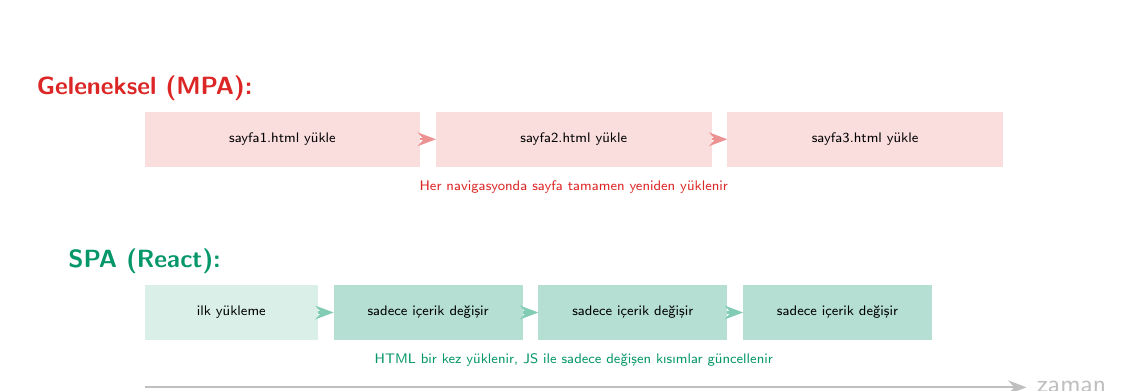
\begin{tikzpicture}[node distance=0.6cm, >=Stealth]

  % Geleneksel
  \node[font=\sffamily\bfseries\small, text=danger] at (0, 4.6) {Geleneksel (MPA):};
  \fill[danger!15] (0.0,3.6) rectangle (3.5,4.3);
  \fill[danger!15] (3.7,3.6) rectangle (7.2,4.3);
  \fill[danger!15] (7.4,3.6) rectangle (10.9,4.3);
  \node[font=\sffamily\tiny] at (1.75, 3.95) {sayfa1.html yükle};
  \node[font=\sffamily\tiny] at (5.45, 3.95) {sayfa2.html yükle};
  \node[font=\sffamily\tiny] at (9.15, 3.95) {sayfa3.html yükle};
  \draw[->, thick, danger!50] (3.5,3.95) -- (3.7,3.95);
  \draw[->, thick, danger!50] (7.2,3.95) -- (7.4,3.95);
  \node[font=\sffamily\tiny\color{danger}, below] at (5.45,3.55) {Her navigasyonda sayfa tamamen yeniden yüklenir};

  % SPA
  \node[font=\sffamily\bfseries\small, text=accent] at (0, 2.4) {SPA (React):};
  \fill[accent!15] (0.0,1.4) rectangle (2.2,2.1);
  \fill[accent!30] (2.4,1.4) rectangle (4.8,2.1);
  \fill[accent!30] (5.0,1.4) rectangle (7.4,2.1);
  \fill[accent!30] (7.6,1.4) rectangle (10.0,2.1);
  \node[font=\sffamily\tiny] at (1.1, 1.75) {ilk yükleme};
  \node[font=\sffamily\tiny] at (3.6, 1.75) {sadece içerik değişir};
  \node[font=\sffamily\tiny] at (6.2, 1.75) {sadece içerik değişir};
  \node[font=\sffamily\tiny] at (8.8, 1.75) {sadece içerik değişir};
  \draw[->, thick, accent!50] (2.2,1.75) -- (2.4,1.75);
  \draw[->, thick, accent!50] (4.8,1.75) -- (5.0,1.75);
  \draw[->, thick, accent!50] (7.4,1.75) -- (7.6,1.75);
  \node[font=\sffamily\tiny\color{accent}, below] at (5.45,1.35) {HTML bir kez yüklenir, JS ile sadece değişen kısımlar güncellenir};

  % Zaman oku
  \draw[->, thick, gray!50] (0.0, 0.8) -- (11.2, 0.8)
    node[right, font=\sffamily\small] {zaman};

\end{tikzpicture}
\end{center}

\vspace{4pt}

\begin{infobox}[\faLightbulb\ SPA Avantajları]
\begin{itemize}
  \item Daha hızlı geçişler --- sayfa yeniden yüklenmez
  \item Daha iyi kullanıcı deneyimi --- masaüstü uygulaması hissi
  \item Frontend ve backend bağımsız geliştirilebilir
\end{itemize}
\end{infobox}

% ----------------------------------------------------------
\subsection{Virtual DOM}

React, gerçek DOM'u doğrudan değiştirmek yerine bellekte bir \textbf{kopya (Virtual DOM)} tutar.
Veri değiştiğinde:

\begin{enumerate}
  \item Yeni Virtual DOM oluşturulur
  \item Önceki ile karşılaştırılır (\textbf{diffing})
  \item Sadece değişen kısımlar gerçek DOM'a uygulanır (\textbf{reconciliation})
\end{enumerate}

\vspace{8pt}

\begin{center}
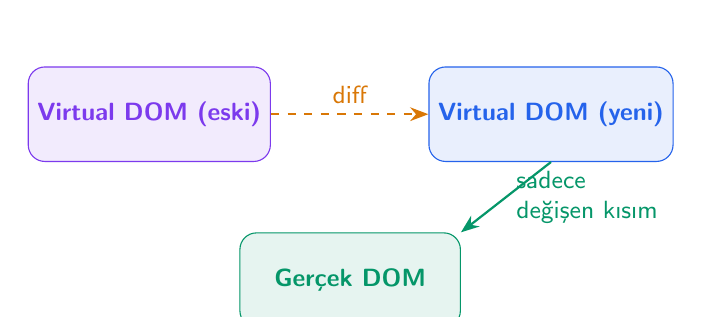
\begin{tikzpicture}[node distance=1.0cm, >=Stealth]

  \node[draw=secondary, fill=secondary!10, rounded corners=6pt,
        minimum width=2.8cm, minimum height=1.2cm,
        font=\sffamily\bfseries\small, text=secondary] (vdom1)
        {Virtual DOM (eski)};

  \node[draw=primary, fill=primary!10, rounded corners=6pt,
        minimum width=2.8cm, minimum height=1.2cm,
        font=\sffamily\bfseries\small, text=primary,
        right=2.0cm of vdom1] (vdom2)
        {Virtual DOM (yeni)};

  \node[draw=accent, fill=accent!10, rounded corners=6pt,
        minimum width=2.8cm, minimum height=1.2cm,
        font=\sffamily\bfseries\small, text=accent,
        below=1.5cm of $(vdom1)!0.5!(vdom2)$] (realdom)
        {Gerçek DOM};

  \draw[->, thick, color=warning, dashed]
    (vdom1.east) -- node[above, font=\small\sffamily, text=warning] {diff} (vdom2.west);

  \draw[->, thick, color=accent]
    (vdom2.south) -- node[right, font=\small\sffamily, text=accent, align=left]
    {sadece\\değişen kısım} (realdom.north east);

\end{tikzpicture}
\end{center}

\begin{warningbox}[\faExclamationTriangle\ Önemli]
Virtual DOM ``hızlı'' olduğundan değil, \textbf{hangi DOM düğümlerinin
değiştiğini verimli hesapladığından} faydalıdır. Tüm sayfayı yeniden
çizmek yerine sadece değişen elemanları günceller.
\end{warningbox}

% ============================================================
\newpage
\section{\faCubes\ Component, JSX ve Props}
\timebadge{20--45 dakika}

\subsection{Component Nedir?}

React'ta her şey \textbf{component}'tir --- yeniden kullanılabilir,
bağımsız UI parçaları. Bir sayfa, iç içe component'lerden oluşur.

\vspace{8pt}

\begin{center}
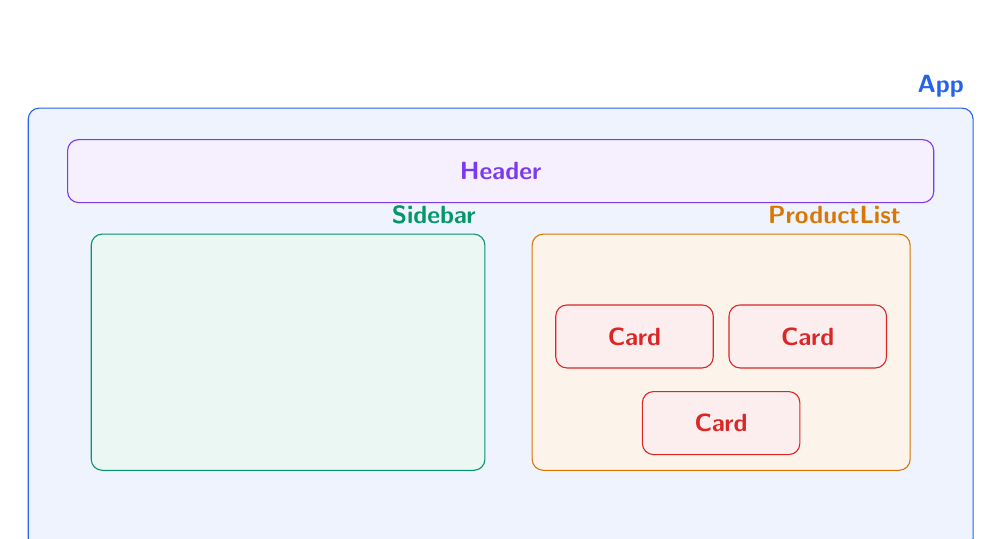
\begin{tikzpicture}[
  box/.style={draw=#1, fill=#1!8, rounded corners=4pt,
    minimum height=0.9cm, font=\sffamily\small\bfseries, text=#1},
  >=Stealth
]
  % App
  \node[box=primary, minimum width=12cm, minimum height=5.6cm] (app) at (0,0) {};
  \node[primary, font=\sffamily\bfseries\small, above left] at (app.north east) {App};

  % Header
  \node[box=secondary, minimum width=11cm, minimum height=0.8cm] (header) at (0,2.0) {Header};

  % Main content area
  \node[box=accent, minimum width=5cm, minimum height=3.0cm] (sidebar) at (-2.7,-0.3) {};
  \node[accent, font=\sffamily\bfseries\small, above left] at (sidebar.north east) {Sidebar};

  % Card components inside main
  \node[box=warning, minimum width=4.8cm, minimum height=3.0cm] (main) at (2.8,-0.3) {};
  \node[warning, font=\sffamily\bfseries\small, above left] at (main.north east) {ProductList};

  \node[box=danger, minimum width=2.0cm, minimum height=0.8cm] (card1) at (1.7,-0.1) {Card};
  \node[box=danger, minimum width=2.0cm, minimum height=0.8cm] (card2) at (3.9,-0.1) {Card};
  \node[box=danger, minimum width=2.0cm, minimum height=0.8cm] (card3) at (2.8,-1.2) {Card};

\end{tikzpicture}
\end{center}

\vspace{6pt}

\begin{definebox}[Component = Fonksiyon]
React'ta bir component, \textbf{JSX döndüren bir JavaScript fonksiyonudur}.
İsmi \textbf{büyük harfle} başlar.
\end{definebox}

\vspace{6pt}

\begin{tcolorbox}[enhanced, colback=codebg, colframe=gray!30,
    colbacktitle=primary!85!black, coltitle=white, arc=4pt,
    title={\sffamily\bfseries\small İlk Component}]
\begin{lstlisting}[style=jsxstyle]
// En basit component
function Greeting() {
  return <h1>Hello, React!</h1>;
}

// Arrow function ile (ayni sey)
const Greeting = () => {
  return <h1>Hello, React!</h1>;
};

// Kullanim
<Greeting />
\end{lstlisting}
\end{tcolorbox}

% ----------------------------------------------------------
\subsection{JSX Nedir?}

JSX, JavaScript içinde HTML yazmamızı sağlayan bir söz dizimidir.
Tarayıcı JSX'i anlamaz; derleme araçları (Babel/SWC) onu normal
JavaScript'e çevirir.

\vspace{6pt}

\begin{tcolorbox}[enhanced, colback=codebg, colframe=gray!30,
    colbacktitle=primary!85!black, coltitle=white, arc=4pt,
    title={\sffamily\bfseries\small JSX vs JavaScript}]
\begin{lstlisting}[style=jsxstyle]
// JSX (developer yazar)
const element = <h1 className="title">Hello</h1>;

// JavaScript (derleyici uretir)
const element = React.createElement(
  "h1",
  { className: "title" },
  "Hello"
);
\end{lstlisting}
\end{tcolorbox}

\vspace{6pt}

\subsubsection{JSX Kuralları}

\begin{tcolorbox}[enhanced, colback=lightbg, colframe=gray!30, arc=4pt]
\sffamily\small
\begin{tabularx}{\textwidth}{>{\bfseries\color{primary}}l X}
\toprule
Kural & Açıklama \\
\midrule
Tek kök eleman &
  Her component \textbf{tek bir üst eleman} döndürmeli.
  Birden fazla eleman varsa \texttt{<div>} veya \texttt{<>...</>} (Fragment) ile sarın. \\[4pt]
\texttt{className} &
  HTML'deki \texttt{class} yerine \texttt{className} kullanılır
  (\texttt{class} JS'te ayrılmış kelimedir). \\[4pt]
Süslü parantez &
  JS ifadeleri \texttt{\{...\}} içinde yazılır: \texttt{\{user.name\}}, \texttt{\{2 + 3\}} \\[4pt]
Self-closing &
  Çocuğu olmayan etiketler kapatılmalıdır: \texttt{<img />}, \texttt{<input />} \\[4pt]
camelCase &
  HTML attribute'ları camelCase olur: \texttt{onClick}, \texttt{onChange}, \texttt{htmlFor} \\
\bottomrule
\end{tabularx}
\end{tcolorbox}

\vspace{6pt}

\begin{tcolorbox}[enhanced, colback=codebg, colframe=gray!30,
    colbacktitle=primary!85!black, coltitle=white, arc=4pt,
    title={\sffamily\bfseries\small JSX Örnekleri}]
\begin{lstlisting}[style=jsxstyle]
function UserCard() {
  const name = "Ali";
  const age = 28;
  const isAdmin = true;

  return (
    <div className="card">
      {/* JS ifadeleri suslu parantez icinde */}
      <h2>{name}</h2>
      <p>Age: {age}</p>
      <p>Role: {isAdmin ? "Admin" : "User"}</p>
    </div>
  );
}
\end{lstlisting}
\end{tcolorbox}

\vspace{4pt}

\begin{warningbox}[\faExclamationTriangle\ Fragment]
Birden fazla eleman döndürmek istiyorsanız, gereksiz \texttt{<div>}
eklemek yerine \textbf{Fragment} kullanın:

\vspace{4pt}
\texttt{<> ... </>} \quad veya \quad \texttt{<React.Fragment> ... </React.Fragment>}
\end{warningbox}

% ----------------------------------------------------------
\newpage
\subsection{Props --- Component'e Veri Aktarımı}

\texttt{Props} (properties), bir component'e \textbf{dışarıdan veri göndermek}
için kullanılır. HTML attribute'larına benzer, ama herhangi bir
JavaScript değeri olabilir.

\vspace{6pt}

\begin{tcolorbox}[enhanced, colback=codebg, colframe=gray!30,
    colbacktitle=primary!85!black, coltitle=white, arc=4pt,
    title={\sffamily\bfseries\small Props Kullanımı}]
\begin{lstlisting}[style=jsxstyle]
// Component tanimlarken props parametresi alinir
function Greeting(props) {
  return <h1>Hello, {props.name}!</h1>;
}

// Daha yaygin: destructuring ile
function Greeting({ name }) {
  return <h1>Hello, {name}!</h1>;
}

// Kullanim --- attribute gibi yazilir
<Greeting name="Ali" />
<Greeting name="Zeynep" />
<Greeting name="Can" />
\end{lstlisting}
\end{tcolorbox}

\vspace{6pt}

\begin{tcolorbox}[enhanced, colback=codebg, colframe=gray!30,
    colbacktitle=primary!85!black, coltitle=white, arc=4pt,
    title={\sffamily\bfseries\small Birden Fazla Prop}]
\begin{lstlisting}[style=jsxstyle]
function ProductCard({ title, price, inStock }) {
  return (
    <div className="card">
      <h2>{title}</h2>
      <p>Price: {price} TL</p>
      <p>{inStock ? "In stock" : "Out of stock"}</p>
    </div>
  );
}

// Kullanim
<ProductCard title="Notebook" price={45} inStock={true} />
<ProductCard title="Pencil" price={5} inStock={false} />
\end{lstlisting}
\end{tcolorbox}

\vspace{6pt}

\begin{center}
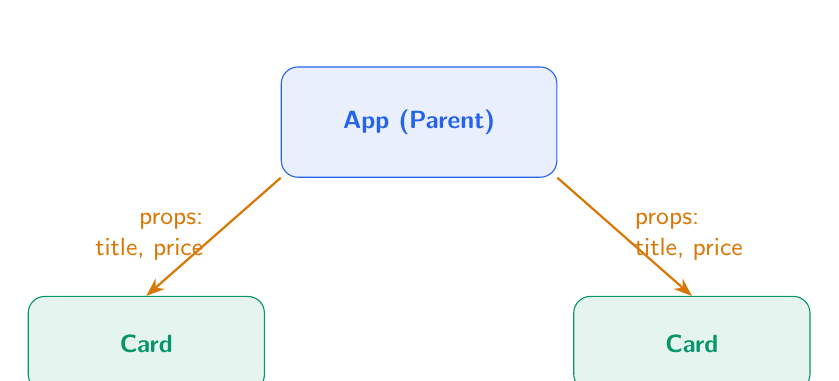
\begin{tikzpicture}[>=Stealth]
  \node[draw=primary, fill=primary!10, rounded corners=6pt,
        minimum width=3.5cm, minimum height=1.4cm,
        font=\sffamily\bfseries\small, text=primary] (parent)
        {App (Parent)};

  \node[draw=accent, fill=accent!10, rounded corners=6pt,
        minimum width=3.0cm, minimum height=1.2cm,
        font=\sffamily\bfseries\small, text=accent,
        below left=1.5cm and 0.2cm of parent] (child1)
        {Card};

  \node[draw=accent, fill=accent!10, rounded corners=6pt,
        minimum width=3.0cm, minimum height=1.2cm,
        font=\sffamily\bfseries\small, text=accent,
        below right=1.5cm and 0.2cm of parent] (child2)
        {Card};

  \draw[->, thick, color=warning]
    (parent.south west) -- node[left, font=\small\sffamily, text=warning, align=right]
    {props:\\ title, price}
    (child1.north);

  \draw[->, thick, color=warning]
    (parent.south east) -- node[right, font=\small\sffamily, text=warning, align=left]
    {props:\\ title, price}
    (child2.north);
\end{tikzpicture}
\end{center}

\vspace{4pt}

\begin{dangerbox}[\faExclamationCircle\ Props Read-Only'dir]
Props \textbf{değiştirilemez}. Bir component aldığı prop'u sadece \textbf{okuyabilir}.
Değişebilir veri için \textbf{state} kullanılır (bir sonraki bölüm).
\end{dangerbox}

% ----------------------------------------------------------
\subsubsection{children Prop'u}

Component'in açılış ve kapanış etiketi arasına yazılan içerik,
otomatik olarak \texttt{children} prop'u ile gelir.

\vspace{6pt}

\begin{tcolorbox}[enhanced, colback=codebg, colframe=gray!30,
    colbacktitle=primary!85!black, coltitle=white, arc=4pt,
    title={\sffamily\bfseries\small children Örneği}]
\begin{lstlisting}[style=jsxstyle]
function Card({ children }) {
  return (
    <div className="card">
      {children}
    </div>
  );
}

// Kullanim
<Card>
  <h2>Product Title</h2>
  <p>Description text here.</p>
</Card>
\end{lstlisting}
\end{tcolorbox}

% ============================================================
\newpage
\section{\faDatabase\ State ve Event Handling}
\timebadge{45--70 dakika}

\subsection{State Nedir?}

\textbf{Props} dışarıdan gelir ve değiştirilemez.
\textbf{State} ise component'in \textbf{kendi içinde tuttuğu değişebilir veridir}.

State değiştiğinde React o component'i \textbf{otomatik olarak yeniden render} eder.

\vspace{6pt}

\begin{center}
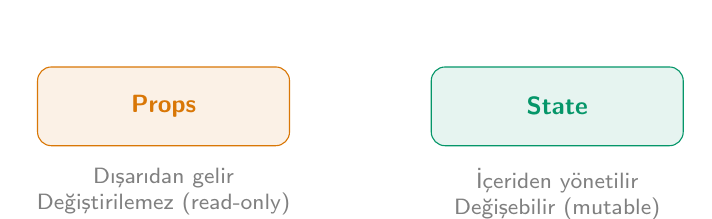
\begin{tikzpicture}[
  box/.style={draw=#1, fill=#1!10, rounded corners=5pt,
    minimum width=3.2cm, minimum height=1.0cm,
    font=\sffamily\small\bfseries, text=#1}
]
  \node[box=warning] (props) at (0, 0) {Props};
  \node[box=accent]  (state) at (5, 0) {State};

  \node[font=\sffamily\footnotesize, text=gray, below=0.15cm of props, align=center]
    {Dışarıdan gelir\\Değiştirilemez (read-only)};
  \node[font=\sffamily\footnotesize, text=gray, below=0.15cm of state, align=center]
    {İçeriden yönetilir\\Değişebilir (mutable)};
\end{tikzpicture}
\end{center}

% ----------------------------------------------------------
\subsection{useState Hook}

\texttt{useState}, React'in en temel Hook'udur. Component'e
\textbf{değişebilir veri} (state) eklememizi sağlar.

\vspace{6pt}

\begin{definebox}[useState Formülü]
\texttt{const [deger, setDeger] = useState(baslangicDeger);}

\begin{itemize}
  \item \texttt{deger} --- state'in şu anki değeri
  \item \texttt{setDeger} --- değeri güncelleyen fonksiyon
  \item \texttt{baslangicDeger} --- ilk render'daki değer
\end{itemize}
\end{definebox}

\vspace{6pt}

\begin{tcolorbox}[enhanced, colback=codebg, colframe=gray!30,
    colbacktitle=primary!85!black, coltitle=white, arc=4pt,
    title={\sffamily\bfseries\small useState --- Basit Counter}]
\begin{lstlisting}[style=jsxstyle]
import { useState } from "react";

function Counter() {
  const [count, setCount] = useState(0);

  return (
    <div>
      <p>Count: {count}</p>
      <button onClick={() => setCount(count + 1)}>
        Increase
      </button>
    </div>
  );
}
\end{lstlisting}
\end{tcolorbox}

\vspace{8pt}

\begin{center}
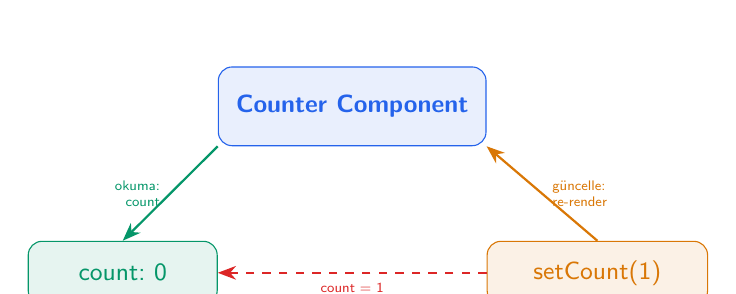
\begin{tikzpicture}[>=Stealth, node distance=1.5cm]

  \node[draw=primary, fill=primary!10, rounded corners=5pt,
        minimum width=3.4cm, minimum height=1.0cm,
        font=\sffamily\bfseries\small, text=primary] (comp)
        {Counter Component};

  \node[draw=accent, fill=accent!10, rounded corners=5pt,
        minimum width=2.4cm, minimum height=0.8cm,
        font=\sffamily\small, text=accent,
        below left=1.2cm and 0.0cm of comp] (state)
        {count: 0};

  \node[draw=warning, fill=warning!10, rounded corners=5pt,
        minimum width=2.8cm, minimum height=0.8cm,
        font=\sffamily\small, text=warning,
        below right=1.2cm and 0.0cm of comp] (setter)
        {setCount(1)};

  \draw[->, thick, accent] (comp.south west) -- node[left, font=\sffamily\tiny, align=right]
    {okuma:\\count} (state.north);

  \draw[->, thick, warning] (setter.north) -- node[right, font=\sffamily\tiny, align=left]
    {güncelle:\\re-render} (comp.south east);

  \draw[->, thick, danger, dashed] (setter.west) -- node[below, font=\sffamily\tiny]
    {count = 1} (state.east);

\end{tikzpicture}
\end{center}

% ----------------------------------------------------------
\newpage
\subsection{Event Handling}

React'ta event'ler (olaylar), HTML'deki gibi attribute olarak yazılır.
Fark: \textbf{camelCase} kullanılır ve fonksiyon referansı verilir.

\vspace{6pt}

\begin{tcolorbox}[enhanced, colback=lightbg, colframe=gray!30, arc=4pt]
\sffamily\small
\begin{tabularx}{\textwidth}{>{\ttfamily\color{primary}}l >{\ttfamily\color{secondary}}l X}
\toprule
\normalfont\bfseries HTML & \normalfont\bfseries React (JSX) & \normalfont\bfseries Açıklama \\
\midrule
onclick    & onClick    & Tıklama \\
onchange   & onChange   & Input değişimi \\
onsubmit   & onSubmit   & Form gönderimi \\
onmouseover & onMouseOver & Mouse üzerine gelme \\
onfocus    & onFocus    & Elemana odaklanma \\
\bottomrule
\end{tabularx}
\end{tcolorbox}

\vspace{6pt}

\begin{tcolorbox}[enhanced, colback=codebg, colframe=gray!30,
    colbacktitle=primary!85!black, coltitle=white, arc=4pt,
    title={\sffamily\bfseries\small Event Handler Örnekleri}]
\begin{lstlisting}[style=jsxstyle]
function Demo() {
  // 1. Inline arrow function
  <button onClick={() => alert("Clicked!")}>
    Click Me
  </button>

  // 2. Separate function (recommended for readability)
  const handleClick = () => {
    console.log("Button clicked!");
  };
  <button onClick={handleClick}>Click Me</button>

  // 3. Event object
  const handleChange = (event) => {
    console.log("Typed:", event.target.value);
  };
  <input onChange={handleChange} />
}
\end{lstlisting}
\end{tcolorbox}

\vspace{6pt}

\begin{warningbox}[\faExclamationTriangle\ Sık Yapılan Hata]
Event handler'a fonksiyon \textbf{referansı} verilir, \textbf{çağrılmaz}:

\vspace{4pt}
\texttt{onClick=\{handleClick\}} \quad\color{accent}\faCheck\ Doğru

\texttt{onClick=\{handleClick()\}} \quad\color{danger}\faTimes\ Yanlış --- render sırasında hemen çalışır!
\end{warningbox}

% ----------------------------------------------------------
\subsection{State ile Input Kontrolü}

React'ta form input'ları genellikle \textbf{controlled component}
olarak kullanılır: input'un değeri state'te tutulur, her değişiklik
\texttt{onChange} ile state'e yazılır.

\vspace{6pt}

\begin{tcolorbox}[enhanced, colback=codebg, colframe=gray!30,
    colbacktitle=primary!85!black, coltitle=white, arc=4pt,
    title={\sffamily\bfseries\small Controlled Input}]
\begin{lstlisting}[style=jsxstyle]
import { useState } from "react";

function SearchBox() {
  const [query, setQuery] = useState("");

  const handleChange = (e) => {
    setQuery(e.target.value);
  };

  return (
    <div>
      <input
        type="text"
        value={query}
        onChange={handleChange}
        placeholder="Search..."
      />
      <p>Searching for: {query}</p>
    </div>
  );
}
\end{lstlisting}
\end{tcolorbox}

\vspace{8pt}

\begin{center}
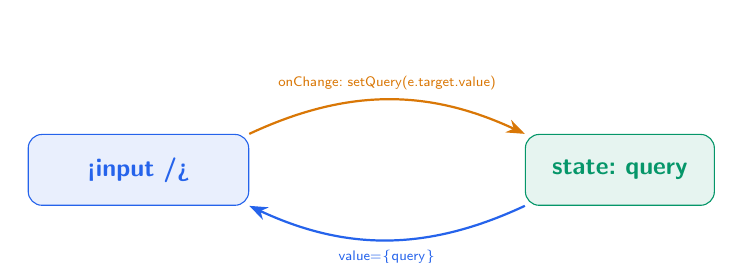
\begin{tikzpicture}[>=Stealth]

  \node[draw=primary, fill=primary!10, rounded corners=5pt,
        minimum width=2.8cm, minimum height=0.9cm,
        font=\sffamily\small\bfseries, text=primary] (input)
        {<input />};

  \node[draw=accent, fill=accent!10, rounded corners=5pt,
        minimum width=2.4cm, minimum height=0.9cm,
        font=\sffamily\small\bfseries, text=accent,
        right=3.5cm of input] (state)
        {state: query};

  \draw[->, thick, warning, bend left=25]
    (input.north east) to
    node[above, font=\sffamily\tiny, text=warning] {onChange: setQuery(e.target.value)}
    (state.north west);

  \draw[->, thick, primary, bend left=25]
    (state.south west) to
    node[below, font=\sffamily\tiny, text=primary] {value=\{query\}}
    (input.south east);

\end{tikzpicture}
\end{center}

\vspace{4pt}

\begin{infobox}[\faLightbulb\ Neden Controlled?]
State tek kaynak (single source of truth) olur. Input'un değerini
her an bilebilir, filtreleyebilir veya doğrulayabiliriz.
React ekosisteminde standart yaklaşım budur.
\end{infobox}

% ============================================================
\newpage
\section{\faHammer\ Pratik: Counter + Listeye Ekleme}
\timebadge{70--90 dakika}

\begin{practicebox}[\faTasks\ Pratik Hedef]
İki mini uygulama oluşturacağız:
\begin{enumerate}
  \item \textbf{Counter:} Artır / Azalt / Sıfırla butonları olan bir sayaç
  \item \textbf{Listeye Ekleme:} Input'tan metin alıp listeye ekleyen uygulama
\end{enumerate}
\end{practicebox}

\vspace{8pt}

% --- Pratik 1: Counter ---
\subsection{Pratik 1 --- Counter Component}

\begin{tcolorbox}[enhanced, colback=codebg, colframe=gray!30,
    colbacktitle=primary!85!black, coltitle=white, arc=4pt,
    title={\sffamily\bfseries\small Counter.jsx}]
\begin{lstlisting}[style=jsxstyle]
import { useState } from "react";

function Counter() {
  const [count, setCount] = useState(0);

  return (
    <div style={{ textAlign: "center", marginTop: 40 }}>
      <h1>Counter: {count}</h1>

      <button onClick={() => setCount(count - 1)}>
        - Decrease
      </button>

      <button onClick={() => setCount(0)}>
        Reset
      </button>

      <button onClick={() => setCount(count + 1)}>
        + Increase
      </button>
    </div>
  );
}

export default Counter;
\end{lstlisting}
\end{tcolorbox}

\vspace{8pt}

% --- Pratik 2: Liste Ekleme ---
\subsection{Pratik 2 --- Input'tan Listeye Ekleme}

\begin{tcolorbox}[enhanced, colback=codebg, colframe=gray!30,
    colbacktitle=primary!85!black, coltitle=white, arc=4pt,
    title={\sffamily\bfseries\small ItemList.jsx}]
\begin{lstlisting}[style=jsxstyle]
import { useState } from "react";

function ItemList() {
  const [items, setItems] = useState([]);
  const [text, setText] = useState("");

  const handleAdd = () => {
    if (text.trim() === "") return;

    setItems([...items, text]);
    setText("");
  };

  return (
    <div style={{ maxWidth: 400, margin: "40px auto" }}>
      <h1>My List</h1>

      <div>
        <input
          type="text"
          value={text}
          onChange={(e) => setText(e.target.value)}
          placeholder="Add an item..."
        />
        <button onClick={handleAdd}>Add</button>
      </div>

      <ul>
        {items.map((item, index) => (
          <li key={index}>{item}</li>
        ))}
      </ul>

      <p>{items.length} items in list</p>
    </div>
  );
}

export default ItemList;
\end{lstlisting}
\end{tcolorbox}

\vspace{6pt}

\begin{infobox}[\faLightbulb\ Neler Kullandık?]
\begin{itemize}
  \item \texttt{useState} ile iki state: dizi (\texttt{items}) ve metin (\texttt{text})
  \item \texttt{spread} ile immutable güncelleme: \texttt{[...items, text]}
  \item \texttt{map} ile liste render
  \item \texttt{onChange} ile controlled input
  \item \texttt{onClick} ile buton event'i
\end{itemize}
\end{infobox}

\vspace{6pt}

\begin{warningbox}[\faExclamationTriangle\ key Prop'u]
\texttt{map} ile liste render ederken her elemana \textbf{benzersiz}
\texttt{key} prop'u verilmelidir. React, hangi elemanın değiştiğini
bulmak için \texttt{key} değerini kullanır.

\vspace{4pt}
İdeal olarak \texttt{key} için veritabanındaki \texttt{id} kullanılır.
\texttt{index} son çare olarak kullanılabilir ama sıralama değişirse
sorun yaratabilir.
\end{warningbox}

% ============================================================
\newpage
\section{\faCheckCircle\ Özet ve Sonraki Session}

\subsection{Bu Session'da Öğrendiklerimiz}

\begin{tcolorbox}[enhanced, colback=lightbg, colframe=gray!30, arc=4pt]
\begin{itemize}
  \item[\color{accent}\faCheck] React nedir ve neden kullanılır
  \item[\color{accent}\faCheck] SPA (Single Page Application) mantığı
  \item[\color{accent}\faCheck] Virtual DOM ve React'in güncelleme mekanizması
  \item[\color{accent}\faCheck] Component = JSX döndüren fonksiyon
  \item[\color{accent}\faCheck] JSX kuralları: tek kök eleman, className, süslü parantez
  \item[\color{accent}\faCheck] Props ile component'e veri aktarımı
  \item[\color{accent}\faCheck] children prop'u
  \item[\color{accent}\faCheck] useState Hook ile state yönetimi
  \item[\color{accent}\faCheck] Event handling: onClick, onChange
  \item[\color{accent}\faCheck] Controlled input patterni
  \item[\color{accent}\faCheck] Pratik: Counter ve listeye eleman ekleme
\end{itemize}
\end{tcolorbox}

\vspace{6pt}

\subsection{Sıkça Sorulan Sorular}

\begin{warningbox}[\faQuestionCircle\ SSS]
\textbf{S: Component isimleri neden büyük harfle başlar?}\\
C: React, küçük harfle başlayan tag'leri HTML elemanı olarak yorumlar
(\texttt{<div>}, \texttt{<p>}). Büyük harfle başlayanlar ise
özel component olarak tanımlanır (\texttt{<Counter />}).

\vspace{6pt}
\textbf{S: State'i neden doğrudan değiştirmiyoruz?}\\
C: \texttt{count = 5} yazsak React bundan haberdar olmaz ve
ekranı güncellemez. \texttt{setCount(5)} dediğimizde React yeni
değeri alır ve component'i yeniden render eder.

\vspace{6pt}
\textbf{S: Her component'in kendi state'i mi var?}\\
C: Evet. Aynı component'ten birden fazla kullanılsa bile her birinin
state'i bağımsızdır. \texttt{<Counter />} iki kez yazılırsa ikisi
birbirini etkilemez.
\end{warningbox}

\vspace{6pt}

\subsection{Sonraki Session --- Session 4: React Derinleşme}

\begin{infobox}[\faArrowRight\ Session 4 (6 Mayıs Çarşamba)]
React bilgimizi proje seviyesine çıkarmak için:
\begin{itemize}
  \item \textbf{useEffect} --- yan etkiler ve lifecycle
  \item \textbf{Conditional rendering} --- koşullu gösterim
  \item \textbf{List rendering} ve \texttt{key} konusu (detaylı)
  \item \textbf{Form handling} --- controlled input, validation
  \item \textbf{Pratik:} Mini ToDo uygulaması
\end{itemize}
\end{infobox}

\vspace{16pt}
\begin{center}
  \color{gray}\sffamily\small
  Front-end + Next.js Eğitimi \quad|\quad Session 3 / 8 \quad|\quad 4 Mayıs 2026
\end{center}

\end{document}
